\documentclass[UTF8]{ctexart}
\usepackage{geometry, CJKutf8}
\geometry{margin=1.5cm, vmargin={0pt,1cm}}
\setlength{\topmargin}{-1cm}
\setlength{\paperheight}{29.7cm}
\setlength{\textheight}{25.3cm}

% 加载TikZ宏包
\usepackage{tikz}
\usetikzlibrary{trees}

\begin{document}

\title{二叉搜索树的删除操作分析报告}
\author{朱孔阳}
\maketitle

\section{Remark}
感谢GPT帮忙用TikZ绘制的二叉树结构图!另外这篇是备用文档,TikZ图的位置没调。

\section{修改后的 remove 函数实现}
detachMin函数用于找到并分离给定子树中的最小节点。而修改后的 `remove` 函数在以下三种情况下处理节点的删除:

\begin{itemize}
  \item 1:被删除节点无子节点。直接删除该节点。
  \item 2:被删除节点有一个子节点。删除该节点并用其子节点替代。
  \item 3:被删除节点有两个子节点。找到右子树中的最小节点并将其值复制到当前节点,然后删除右子树中的最小节点。
\end{itemize}



\section{测试输出结果的呈现和分析}

初始树结构如下:
\begin{tikzpicture}[sibling distance=5em, level distance=8em, 
  every node/.style = {shape=rectangle, rounded corners, draw, align=center}]
  \node {5}
    child {node {3}
      child {node {2} edge from parent node [left] {/}}
      child {node {4} edge from parent node [right] {\\}}
    }
    child {node {7}
      child {node {6} edge from parent node [left] {/}}
      child {node {8} edge from parent node [right] {\\}}
    };
\end{tikzpicture}

移除元素 3 后:
\begin{tikzpicture}[sibling distance=5em, level distance=8em, 
  every node/.style = {shape=rectangle, rounded corners, draw, align=center}]
  \node {5}
    child {node {2} edge from parent node [left] {/}}
    child {node {7}
      child {node {4} edge from parent node [left] {/}}
      child {node {6} edge from parent node [right] {/}}
      child {node {8} edge from parent node [right] {\\}}
    };
\end{tikzpicture}

移除元素 5 后:
\begin{tikzpicture}[sibling distance=5em, level distance=8em, 
  every node/.style = {shape=rectangle, rounded corners, draw, align=center}]
  \node {7}
    child {node {2} edge from parent node [left] {/}}
    child {node {6}
      child {node {4} edge from parent node [left] {/}}
      edge from parent node [right] {\\}}
    child {node {8} edge from parent node [right] {\\}};
\end{tikzpicture}

移除元素 8 后:
\begin{tikzpicture}[sibling distance=5em, level distance=8em, 
  every node/.style = {shape=rectangle, rounded corners, draw, align=center}]
  \node {7}
    child {node {2} edge from parent node [left] {/}}
    child {node {6}
      child {node {4} edge from parent node [left] {/}}
      edge from parent node [right] {\\}};
\end{tikzpicture}

从测试结果可以看出,每次删除操作后,任意节点的左子树只包含小于该节点的值,右子树只包含大于该节点的值。这表明修改后的 `remove` 函数正确。

\end{document}
